%%%%%%%%%%%%%%%%%%%%%%%%%%%%%%%%%%%%%%%%%
% FRI Data Science_report LaTeX Template
% Version 1.0 (28/1/2020)
%
% Jure Demšar (jure.demsar@fri.uni-lj.si)
%
% Based on MicromouseSymp article template by:
% Mathias Legrand (legrand.mathias@gmail.com)
% With extensive modifications by:
% Antonio Valente (antonio.luis.valente@gmail.com)
%
% License:
% CC BY-NC-SA 3.0 (http://creativecommons.org/licenses/by-nc-sa/3.0/)
%
%%%%%%%%%%%%%%%%%%%%%%%%%%%%%%%%%%%%%%%%%


%----------------------------------------------------------------------------------------
%	PACKAGES AND OTHER DOCUMENT CONFIGURATIONS
%----------------------------------------------------------------------------------------
\documentclass[fleqn,moreauthors,10pt]{ds_report}
\usepackage[english]{babel}

\graphicspath{{figures/}}




%----------------------------------------------------------------------------------------
%	ARTICLE INFORMATION
%----------------------------------------------------------------------------------------

% Header
\JournalInfo{UL FRI - Biomedical signal and image processing}

% Type of report
\Archive{Assigment 2 Report}

% Article title
\PaperTitle{QRS complex classification (normal, abnormal) using a norm of linear algebra or correlation coefficient}

% Authors and their info
\Authors{Aljaz Mur Erzen\textsuperscript{1}}
\affiliation{\textsuperscript{1}\textit{ae4664@student.uni-lj.si, 63160011}}

% Keywords
\Keywords{hearbeat, detection, signal}
\newcommand{\keywordname}{Keywords}


%----------------------------------------------------------------------------------------
%	ABSTRACT
%----------------------------------------------------------------------------------------

%----------------------------------------------------------------------------------------

\begin{document}

% Makes all text pages the same height
\flushbottom

% Print the title and abstract box
\maketitle

% Removes page numbering from the first page
\thispagestyle{empty}

%----------------------------------------------------------------------------------------
%	ARTICLE CONTENTS
%----------------------------------------------------------------------------------------

\section*{Introduction}
	
Automatic heartbeat classification plays a key role in analyzing streams of recorded ECG signals, finding abnormalities and predicting possible heart diseases. Due to significance of the implications, there is a lot of motivation to improve performance of existing classification algorithms.

This report describes how we implemented a simple classification algorithm based on beat comparison to a normal heartbeat using different algebraic norms and a correlation coefficient. The algorithm requires recorded ECG signal and detected R-peaks or QRS complex.

%------------------------------------------------

\section*{Baseline drift suppression}

Due to baseline drift, which is caused by external factors during ECG recording, the signals of the complexes may contain different low frequency signals. This problem can be solved using different approaches:
\begin{description}
	\item[High-pass filters] could suppress the baseline drift, but may also introduce non-linear phase shift, which would distort the QRS complex, lowering probability it would be classified correctly. To remove this phase shift, we could apply the filter \textit{in reverse direction}, but this solution can be done only on pre-recorded signals and not in real-time.
	\item[Isoelectric level offset] If we assume that the baseline drift is constant over one heartbeat, we can align the complexes by simple  subtraction. The offset, which is called isoelectric level of the QRS complex, can be estimated by averaging a few samples before the R-peak or using some other more sophisticated algorithm \cite{iso_estimation}. 
\end{description}

\noindent
Our algorithm uses two variations of the second approach:
\begin{itemize}
	\item isoelectric level estimation which uses sample average of points 72ms, 68ms, 64ms and 60ms before R-peak as the offset.
	\item normalization using the whole signal average and scaling to normalize standard divination.
\end{itemize}

\section*{Computing the normal heartbeat}

To compare the heartbeats, we need a notion of a \textit{normal} heartbeat. The simplest approach is to take first $N$ detected heartbeats and compute their average. This approach may produce bad results if some or all of these beats turn out not to be classified as normal. But in most cases, when the first $N$ QRS complexes are normal, the produced mean signal should be similar to our notion of a normal QRS complex. 

\begin{figure}[ht]\centering
	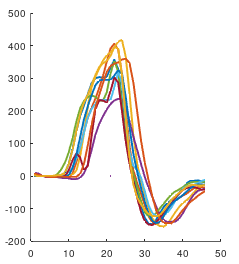
\includegraphics[width=0.49\linewidth]{mean_beat_stacked_iso_est.png}
	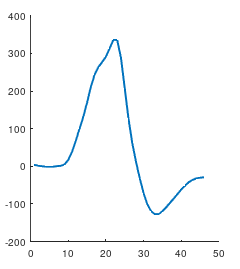
\includegraphics[width=0.49\linewidth]{mean_beat_mean_iso_est.png}
	\caption{\textbf{Overlaid and averaged QRS complexes} 10 ECG signals of the QRS complexes were aligned to match their isoelectric levels. PR segments are therefore well aligned, but R and S peaks are not.}
	\label{fig:mean_beat_iso_est}
\end{figure}

For our implementation, we used 500 first heartbeats, which is about 5 minutes of the signal.

\section*{ECG signal distance}

Now we can compare each detected heartbeat to the \textit{normal} heartbeat. This is done by computing a \textit{distance} measure between the two and then applying a threshold.

We explored four different measures, namely $\ell_1$ norm, Euclidean distance (or $\ell_2$ norm), maximum norm (or $\ell_\infty$ norm) and intra-class correlation coefficient. To obtain best results, the measure and the threshold should be chosen carefully.
\begin{figure}[ht]\centering
	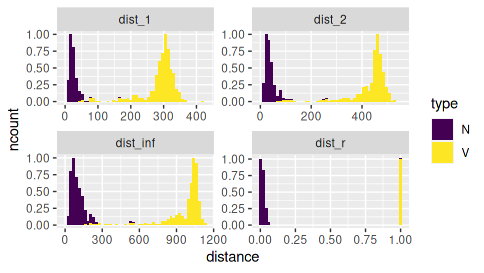
\includegraphics[width=\linewidth]{distances-s20501.png}
	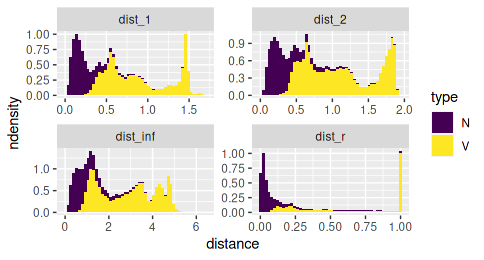
\includegraphics[width=\linewidth]{distances.png}
	\caption{\textbf{Comparison of different distance measures} Plots show distributions of distances to mean heartbeat using different measures. Note that densities are scaled individually for normal (N) and PVC (V) complexes. Upper plot represents record s20501, lower represents the whole LTST database.}
	\label{fig:distance-measures}
\end{figure}

\newpage
To choose the most appropriate threshold, we can plot ROC curve (Receiver Operating Characteristic), which shows different thresholds in FPR-TPR space.

\begin{figure}[!hb]\centering
	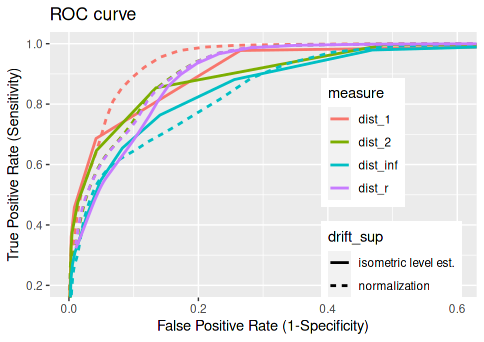
\includegraphics[width=\linewidth]{roc.png}
	\caption{\textbf{ROC curve} Overall, $\ell_1$ norm yields best results. Drift suppression should be chosen based on desired ratio between FPR and TPR.}
	\label{fig:roc}
\end{figure}

\section*{Implementation and testing}
\newpage

Algorithm was implemented in Matlab programming language and used Bash scripts and Physionet's WFDB toolkit \cite{wfdb} for preparing, converting input data and evaluating classifier output. The algorithm was developed and tested on data from LTST database \cite{ltst} containing 86 records each containing 2 or 3 ECG signals with mean duration 23.1h (std = 3.03h).

On a desktop computer with processor Processor AMD Ryzen 5 1600 Six-Core and Matlab version 9.9.0, mean running time of the classifier analyzing one of the records was 1.53s (std = 0.25s), but real running time (including Matlab startup and annotation reading) was 16.81s (std = 3.48s).

\section*{Results}

With selected $\ell_1$ norm, signal normalization for drift suppression and threshold of $0.43$, the algorithm achieved following results:
\begin{table}[hbt]
	\centering
	\begin{tabular}{l | r}
		\toprule
		Beats             & 8708579  \\
		FN                & 6786     \\
		FP                & 933422   \\
		Sensitivity (Se)  & 90.65\%  \\
		Precision (P+) 	  & 6.58\%   \\
		Specificity (Sp)  & 89.19\%  \\
		\bottomrule
	\end{tabular}
	\label{tab:label}
\end{table}
Negative prediction is associated with normal heartbeat (N notation in LTST) and positive prediction is associated with PVC (V notation in LTST).

Due to low ratio between positives and negatives, the precision (or positive predictively P+) is low, even though sensitivity and specificity are relativity high.

Considering that $Se$ and $Sp$ metrics can be chosen arbitrarily from the ROC curve by adjusting the threshold, we could adapt the algorithm to the use case, but combined metrics are still too low for the algorithm to be considered reliable.

One possible improvement is further alignment of the QRS signal; from the figures above we can see that the R and S-peaks are not well aligned, which may be leading cause for high FNR.

\bibliographystyle{unsrt}
\bibliography{report}


\end{document}
